\section{Task 9 - Persistent Credentials}
\subsection{The task}
The credentials are mantained as long as the webapp is running. When shutdown, they should be saved to a file and recovered at the next redeploy.
\subsection{Servlet Context Listener}
We can execute actions when the servlet is turned on or off with the servlet context listener, which uses two methods: \textit{contextInitialized} and \textit{contextDestroyed}.
\subsubsection{ContextListener.java}
When the servlet is turned on, we read the data from the file. If the file does not exist or the file cannot be opened, we create a new context with the admin and another starting user; otherwise we add to the context the users we read.

When the servlet is turned off, we save all the user credentials saved in the context inside the file.


\subsubsection{Screenshots}
\begin{figure}[H]
  \centering
  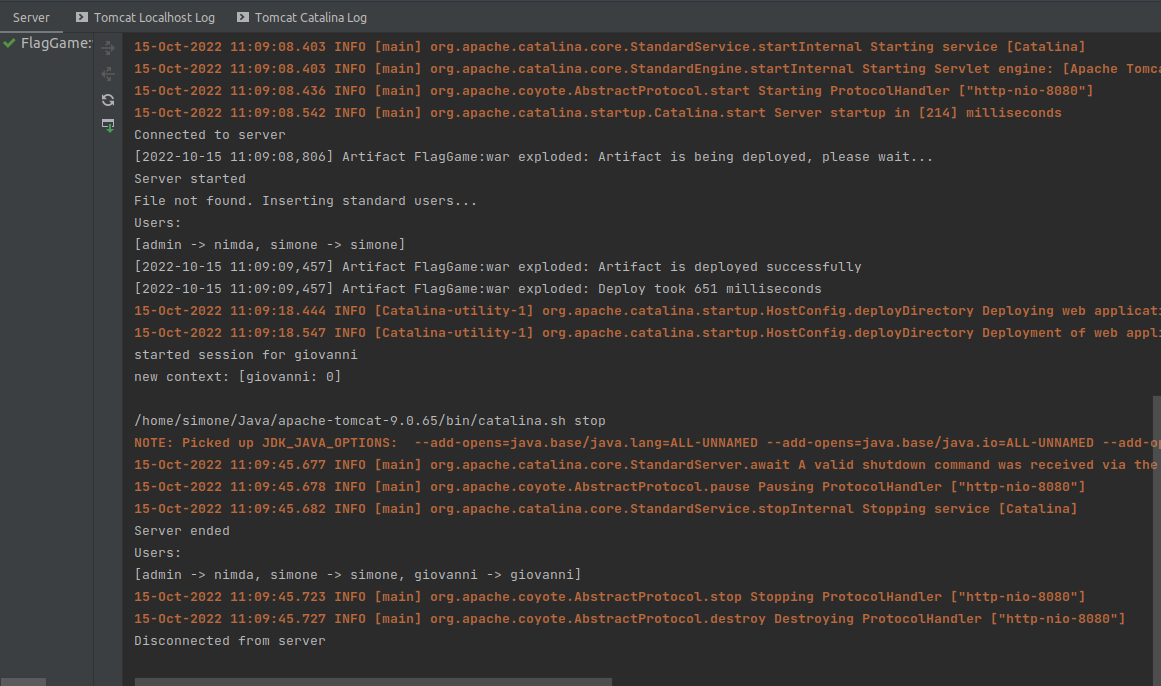
\includegraphics[width=\columnwidth]{context_new.png}
  \caption{When the file is not found, a standard context is created. We then create a new User, and we can see how it also get saved at the server shutdown}
\end{figure}
\begin{figure}[H]
  \centering
  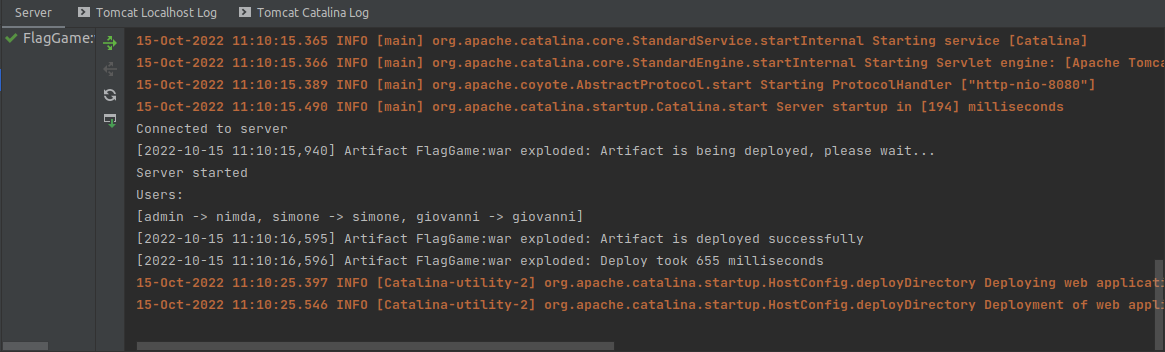
\includegraphics[width=\columnwidth]{context_read.png}
  \caption{At the next redeploy, the three users get correctly recovered}
\end{figure}